\chapter{Arquitetura de solução}
\section{Arquitetura da solução apresentada}
A arquitetura da solução proposta será baseada, de uma forma geral, na arquitetura \ac{mvc}. Este modelo é apresentado em camadas que separam a apresentação e a interação de dados no sistema. É estruturado em três componentes: O modelo é responsável pelo gerenciamento dos dados, a visão que gerencia a apresentação dos dados e o controlador, responsável por intermediar a comunicação entre os eventos gerados pelo usuário na interface e o modelo \cite{engenharia-de-software:2018}

O diagrama apresentado pela Figura 2, mostra o modelo arquitetural adotado.

\begin{figure}[htb]
    \centering
	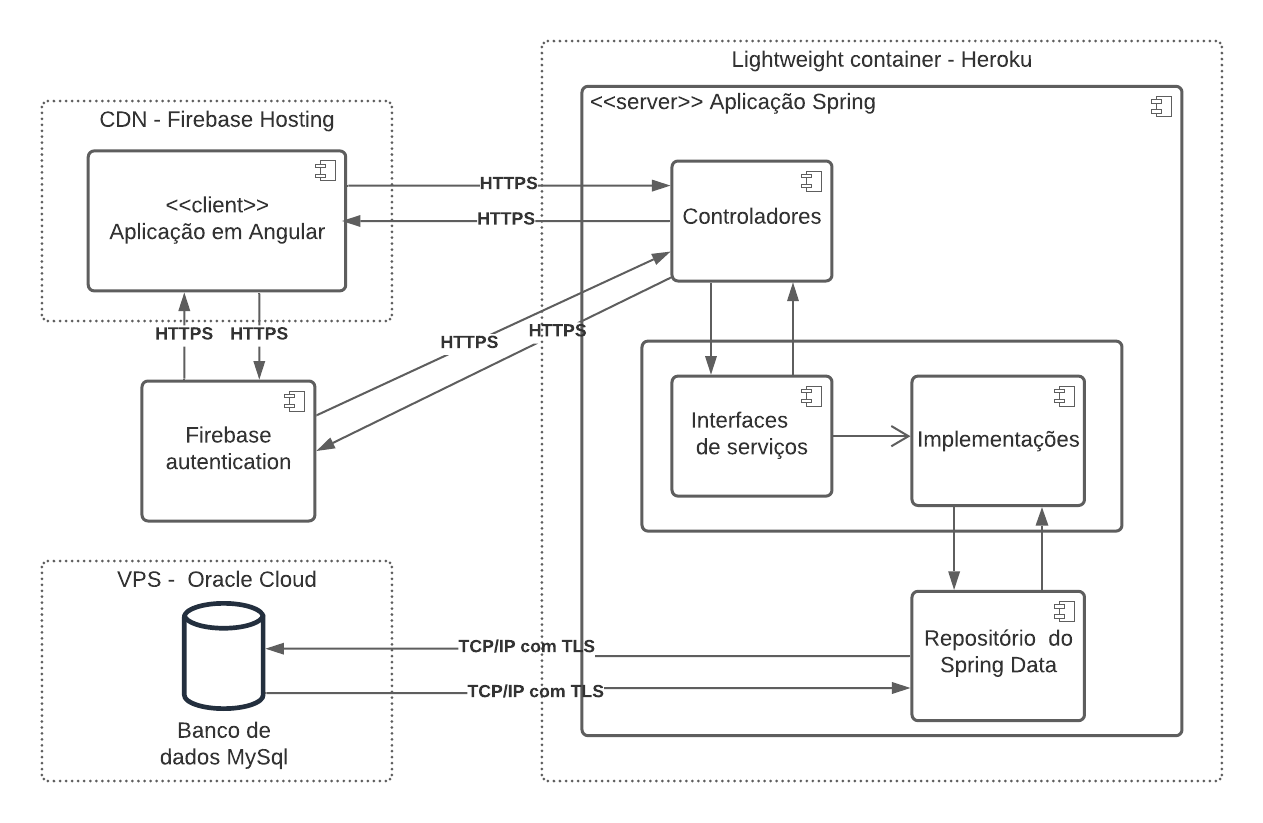
\includegraphics[width=16cm]{imagens/figura2.png}
	\caption{\label{fig_logo} Arquitetura da solução}
	\fonte{Os autores}
\end{figure}
 
 
De modo a desenvolver uma aplicação que busca garantir uma boa usabilidade, e capaz de aproveitar os recursos disponíveis da melhor forma, para a interface do usuário (\textit{\gls{front-end}}) será adotado o modelo arquitetural Single Page Aplication (\ac{spa}). 


Neste modelo, a maioria dos recursos necessários é carregada na inicialização da aplicação, fazendo com que não seja necessário recarregar a página durante o uso. A única mudança que ocorre é a dos dados, que são trafegados entre o servidor e o cliente.


Conforme o diagrama apresentado pela Figura 2, as camadas que compões a solução utilizam as seguintes infraestruturas para hospedagem:
\begin{itemize}
\item \ac{cdn} (Firebase Hosting): infraestrutura responsável por hospedar a aplicação em Angular, da camada de visão. Um serviço de hospedagem, que tem como base o armazenamento em \ac{ssd} e uma \ac{cdn}, totalmente gerenciado para conteúdo estático e dinâmico.
\item  Lightweight container (Heroku): infraestrutura responsável por hospedar a aplicação Spring, da camada controladora. A tecnologia utilizada pelo Heroku, utiliza o conceito de \textit{\gls{container}} que empacota o código e as dependências do aplicativo abstraindo o gerenciamento do \textit{\gls{hardware}}, levando a simplificação do desenvolvimento e o aumento da produtividade.
\item \ac{vps} (Oracle Cloud): infraestrutura responsável por hospedar o banco de dados da aplicação. Esta infraestrutura oferece um alto poder de computação e segurança.
\end{itemize}
Para a autenticação da aplicação, será utilizado o Firebase Authentication. Essa tecnologia oferece o serviços, \ac{sdk} e bibliotecas prontas para autenticar usuários. Sabe-se que a utilização deste serviço trará a aplicação a característica de \textit{\gls{vendor-lock-in}}, isto é, dependente de uma tecnologia terceira.  Porém, as vantagens ofertadas de segurança e a facilidade de implementação levaram a sua adoção ao projeto. 

Ademais, para minimizar os impactos negativos da utilização de uma tecnologia terceira, o Firebase Authentication será implantado seguindo o padrão de projeto \textit{Adapter}. Deste modo, diante da necessidade, a tecnologia poderá ser facilmente substituída por outra ou até mesmo por uma proprietária.


\section{Arquitetura de comunicação entre as camadas}
A comunicação entre a camada de visão e a camada controladora, será realizada via protocolo \ac{https}. Este protocolo acrescenta uma camada a mais de segurança à aplicação, uma vez que utiliza a criptografia na transferência de recursos.


Já a comunicação entre os controladores e banco de dados, será realizada via TCP/IP acrescido do protocolo \ac{tls} que aumenta a segurança através de criptografia, a interoperabilidade, a extensibilidade e a eficiência;


\section{Necessidade de escalabilidade}
A escalabilidade da aplicação estará intimamente ligada à infraestrutura adotada. Como aplicação será hospedada utilizando serviços de nuvem como Heroku e Firebase Hosting, categorizados como \ac{paas}. Os detalhes de infraestrutura são abstraídos facilitando a manutenção, extensão e escalabilidade além de oferecer baixo custo inicial. 

Como a princípio a aplicação será ofertada a um número pequeno de usuários, o plano  gratuito já será suficiente para comportar o número de acessos. E assim, conforme a necessidade será possível escalar a aplicação mediante a contratação de pacotes com mais recursos.